\documentclass[UTF8]{ctexart}
\usepackage{amsmath}
\usepackage{amssymb}
\usepackage{booktabs}
\usepackage{background}
\usepackage{caption,subcaption}
\usepackage{CJKfntef}
\usepackage{cprotect}
\usepackage{enumitem}
\usepackage{fancyhdr}
\usepackage{float}
\usepackage{fontspec}
%\usepackage{fourier}
\usepackage{geometry}
\usepackage{listings}
\usepackage{tikz}
\usetikzlibrary{arrows.meta}
\usepackage{xcolor}

\geometry{a5paper, top=0.1cm, left=1cm, right=1cm, bottom=1cm, footskip=0.1cm}
\setCJKmainfont[BoldFont={汉仪文黑-85W},ItalicFont={方正苏新诗柳楷简体}]{汉仪文黑-55W}
\setfontfamily\Issue{Century Schoolbook}
\setfontfamily\Genshin{Genshin Teyvat Lingua Franca}
\newCJKfontfamily\TitleFont{思源宋体 CN Heavy}
\newfontfamily\timesnewroman{Times New Roman}
%\reversemarginpar

\pagestyle{fancy}
\fancyhf{}
\cfoot{\sffamily\footnotesize{-\ \thepage\ -}}
%\CTEXsetup[format = {\centering\bfseries\large}, beforeskip = 3pt, afterskip = 3pt]{section}

\colorlet{darkcyan}{cyan!50!black}
\newcommand\Black[1]{\textcolor[gray]{0.3}{#1}}
\newcommand\Brown[1]{\textcolor[HTML]{998A4E}{#1}}
\newcommand\Emph[1]{\colorbox{green!10}{\textcolor{green!30!black}{#1}}}
\newcommand\Notes[1]{\textcolor{yellow!50!black}{\small #1}}
\newcommand\Example[1]{\textcolor{cyan!70!black}{\small #1}}

\renewcommand\d{\mathrm{d}}

\lstset{
    basicstyle=\small\ttfamily, %注意行末有逗号!
    keywordstyle=\bfseries\color{blue!70!black},
    commentstyle=\color{cyan!90!black},
    stringstyle=\color{green!40!black},
    columns=flexible,
    numbers=left,
    numberstyle=\footnotesize,
    escapechar=`,
    frame=shadowbox,
    %rulesepcolor=\color{red!20!blue!20!green!20}
    backgroundcolor=\color{cyan!5!white},
    language=C,
    tabsize = 4,
    breaklines = true,
}

\newcommand\IssueNumber{30}
\newcommand\Date{2024-6-8}
%\newcommand\Contributer{@金光日}
\newcommand\Subject{C++ 编程}


\begin{document}
\backgroundsetup{contents=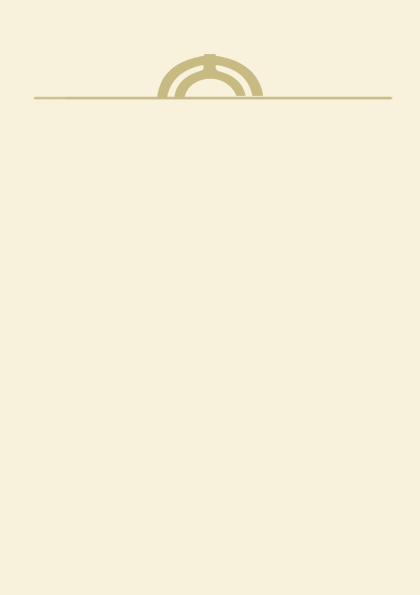
\includegraphics{上半示例.png}, center, scale=1, angle=0, opacity=1}
\BgThispage
\begin{center}
%{\scriptsize\Issue \textcolor[HTML]{C8BA83}{\Genshin WEEKLY TIPS}}
\phantom{...}

{\Large\textcolor{brown!40!white}{\makebox[10cm][s]{\Genshin WEEKLY KNOWLEDGE TIPS}}}

\vspace{-2em}

{\Huge\bfseries\TitleFont \Black{知\ 识\ 小\ 料}}


\vspace{-0.1cm}
{\footnotesize \Brown{「电计 2203 班」周常规知识整理共享}}
\end{center}

\vspace{-0.5cm}


\begin{figure}[H]
\hspace{1cm}
\begin{minipage}[t]{0.3\textwidth}
\centering
    \Brown{\Genshin ISSUE}

    \vspace{-0.6cm}
    \Huge \Issue\slshape\bfseries\Black{\IssueNumber}
\end{minipage}
\hfill
\begin{minipage}[t]{0.35\textwidth}
\centering
    \Brown{日期:\Date} \\
%\vspace{-0.1cm}
%    \Brown{贡献者:\Contributer} \\
\vspace{-0.1cm}
    \Brown{学科:\Subject} \\
\end{minipage}
\hspace{0.8cm}
\end{figure}

{\color{cyan!50!black}
\begin{center}
    C++ STL 总结(上)
\end{center}
STL 是一个功能非常强大的容器库,有许多内置的数据结构与算法实现。也许你在学过了 \verb!queue!、\verb!vector! 以后,就再也不想手写队列了。以下的内容偏向于具体实现。
}

现安利一个「万能头文件」:\cprotect\Emph{\verb!#include<bits/stdc++.h>!},这个头文件可以代替以下所有容器库的头文件。

\section{变长数组:vector}
头文件:\verb!#include<vector>!

vector 本义为「向量」,可理解为可变长的数组,支持随机访问。

\paragraph{声明}  vector 使用以下方法来声明。

\begin{lstlisting}[numbers=none]
#include<vector>  //这是头文件
vector <int> a;   //可变长int数组
vector <int> b[10]; //第一维长度固定为10,第二维长度可变的int数组
struct rec{...};
vector <rec> c;  //自定义的结构体也可以用它来保存
\end{lstlisting}

\paragraph{获知大小与清空} 我们假设 \verb!vector <int> a!。\textcolor{cyan}{(语句有分号代表独立成句,无分号代表一个数值)}
\begin{table}[H]
  \centering
  \begin{tabular}{ll}
  \verb!a.size()! & 返回变长数组 $a$ 的实际长度(元素个数) \\
  \verb!a.empty()! & 返回变长数组 $a$ 是否为空的指示,空返回 1,非空返回 0 \\
  \verb!a.clear();! & 清空变长数组 $a$ \\
  \end{tabular}
\end{table}

\paragraph{插入删除} 我们假设 \verb!vector <int> a!,用以下方法插入、删除元素。
\begin{table}[H]
  \centering
  \begin{tabular}{ll}
  \verb!a.push_back(x);! & 把元素 $x$ 插入到变长数组 $a$ 的末尾 \\
  \verb!a.pop_back();! & 删除变长数组 $a$ 的最后一个元素 \\
  \verb!a.insert(it, x);! & 把元素 $x$ 插入到迭代器 $it$ 的前一个位置 \\
  \verb!a.insert(a.begin(), x);! & 把元素 $x$ 插入到变长数组 $a$ 的开头 \\
  \end{tabular}
\end{table}

\backgroundsetup{contents=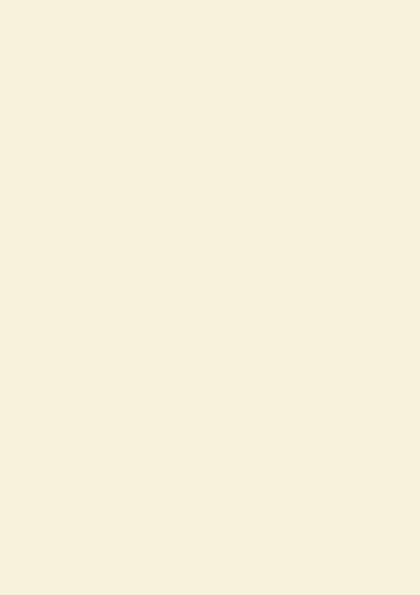
\includegraphics{空白示例.png}, center, scale=1, angle=0, opacity=1}
\BgThispage

\paragraph{查找元素} vector 的吸引人的性质在于它能\Emph{随机存取}元素。
\begin{table}[H]
  \centering
  \begin{tabular}{ll}
  \verb!a[i]! & 随机访问 $a$ 的第 $i$ 个元素,下标从0开始 \\
  \verb!a.front()! & 访问 $a$ 的第一个元素,即 \verb!a[0]! \\
  \verb!a.back()! & 访问 $a$ 的最后一个元素,即 \verb!a[a.size()-1]! \\
  \end{tabular}
\end{table}

以下的语句输出整型变长数组 $a$ 的所有元素:
\begin{lstlisting}[numbers=none]
for(int i=0; i<a.size(); i++)
    printf("%d\n", a[i]);
\end{lstlisting}

\paragraph{迭代器} 遍历 vector 除了采用上面的代码,还可以采用「迭代器」来遍历。迭代器就像 STL 容器的「指针」。正如大一 C 语言程序设计课学的那样,使用 \verb!*! 操作符来取指针指向的值。

\begin{figure}[htb]
  \begin{minipage}[t]{.5\textwidth}
  \centering
  \vspace{0pt}
    \begin{tikzpicture}[>=Stealth]
        \foreach \i in {0,1,...,4}{
            \filldraw[fill=cyan!10] (\i,0) rectangle (\i+1,1);
            \node at (\i+0.5, 0.5) {$a_{\i}$};
        }
        \draw[dashed] (5,0) rectangle (6,1);
        \draw[->] (0.5, -0.5) node[below, font=\footnotesize] {\texttt{a.begin()}} -- (0.5, 0);
        \draw[->] (5.5, -0.5) node[below, font=\footnotesize] {\texttt{a.end()}} -- (5.5, 0);
        \draw[->,blue] (0.5, 1.5) node[above, font=\footnotesize] {\texttt{it}(迭代器)} -- (0.5, 1);
    \end{tikzpicture}
  \end{minipage}
  \begin{minipage}[t]{.48\textwidth}
      \vspace{0pt}
      \centering
      \begin{tabular}{ll}
        \verb!*a.begin()! & 表示 $a_0$ \\
        \verb!*(--a.end())! & 表示 $a_4$ \\
        \verb!*a.end()! & 越界访问 \\
        \verb!*it! & 图中表示 $a_0$ \\
      \end{tabular}
  \end{minipage}
 
%  \begin{minipage}[t]{.61\textwidth}
%  \phantom{...}
%
%  \end{minipage}
%  
  \caption{vector迭代器图解}\label{fig:vector-iterator}
\end{figure}

迭代器使用这种方法声明:
\begin{lstlisting}[numbers=none]
vector<int>::iterator it; //声明整型变长数组的一个迭代器
vector<char>::iterator it1; //声明字符型变长数组的一个迭代器
\end{lstlisting}

\begin{table}[H]
  \centering
  \begin{tabular}{ll}
    \verb!it = a.begin();!  & 让 $it$ 指向变长数组 $a$ 的第一个元素 \\
    \verb!it++;! 或 \verb!it--;!  & 让迭代器 $it$ 向后(或向前)迭代 \\
    \verb!*it! & 取迭代器 $it$ 所指向的值 \\
  \end{tabular}
\end{table}

以下的语句同样输出整型变长数组 $a$ 的所有元素:
\begin{lstlisting}[numbers=none]
vector<int>::iterator it; //声明迭代器 it
for(it = a.begin(); it != a.end(); it++) //让 it 遍历整个变长数组 a
    printf("%d\n", *it);
\end{lstlisting}

\paragraph{实例 1} 输出 2 至 100 的所有质数。
\begin{lstlisting}
#include<bits/stdc++.h>
using namespace std;
bool isPrime(int x){ //判断 x 是否为质数,是则返回1,否则返回0
	for(int i=2; i*i<=x; i++)
		if(x%i==0)
			return 0;
	return 1;
}
int main(){
	vector <int> a; //声明变长数组a
	for(int i=2; i<=100; i++){
		if(isPrime(i))
			a.push_back(i); //如果i是质数则在a的末尾插入i
	}
	int n = a.size(); //数组大小
	cout<<"直接遍历法:"<<endl;
	for(int i=0; i<n; i++)
		cout<<a[i]<<',';
	cout<<endl<<"迭代器遍历法:"<<endl;
	for(vector<int>::iterator  it = a.begin(); it != a.end(); it++)
		cout<<*it<<',';
    return 0;
}
\end{lstlisting}

\paragraph{实例 2} 升序输出给定数字的所有因数,比如 12 的因数有 $\{1,2,3,4,6,12\}$。

\begin{lstlisting}
#include<bits/stdc++.h>
using namespace std;
int main(){
	vector <int> a; //声明变长数组a
	int x;
	scanf("%d",&x);
	for(int i=1; i*i <= x; i++){
		if(x%i == 0){ // i 能整除 x
			a.push_back(i);
			if(i*i !=x) //平方数只插入一次,非平方数要插入i和x/i
				a.push_back(x/i);
		}
	}
	sort(a.begin(), a.end()); //对a进行排序(后面提到)
	for(int i=0; i < a.size(); i++)
		printf("%d ",a[i]);
	return 0;
}
\end{lstlisting}

\section{栈:stack}
头文件:\verb!#include<stack>!

栈是一种先进先出的数据结构。使用下面的方法声明一个栈:
\begin{lstlisting}[numbers=none]
stack<int> s;  //整数值栈
stack<char> s1; //字符值栈
\end{lstlisting}

假设有 \verb!stack<int> s;! 即 $s$ 是一个整型栈。 
\begin{table}[H]
  \centering
  \begin{tabular}{ll}
    \verb!s.size()! & 返回栈 $s$ 的大小 \\
    \verb!s.empty()! & 返回栈 $s$ 是否为空的指示,空返回 1,非空返回 0 \\
    \verb!s.push(x);! & 元素 $x$ 入栈 \\
    \verb!s.pop();! & 出栈 \\
    \verb!s.top()! & 返回栈顶元素 \\
  \end{tabular}
\end{table}

提醒:在使用 \verb!s.pop();! 和 \verb!s.top()! 时,要记得\Emph{对栈是否为空作出检查}。如果对空栈做如此操作,那么编译时不会提醒,但是运行时会出错!

\paragraph{实例} 后缀表达式的计算。输入一个后缀表达式,输出对应值,如输入中缀表达式 $((1-2)\times 3-1)\div 4$ 对应的后缀表达式 \verb!12-3*1-4/!,输出 $-1$。简单起见,程序规定所有数字都是一位数且必能整除。

\begin{lstlisting}
#include<bits/stdc++.h>
using namespace std;
int main(){
	stack<int> s;
	char a[100];
	scanf("%s", a);
	for(int i=0; i<strlen(a); i++){
		if(a[i]>='0' && a[i]<='9') //字符串a的第i位为数字
			s.push(a[i]-'0');
		else{ //字符串a的第i位为符号
			int b[2]; //b[0]和b[1]是两个操作数
			for(int j=0; j<=1; j++){
				if(!s.empty()){ //对空栈作检查,防止运行时错误
					b[j] = s.top(); //取栈顶元素并退栈
					s.pop();
				}
				else{
					printf("表达式有误");
					return 0;
				}
			}
			switch(a[i]){ //后取的元素在前,先取的元素在后,计算结果入栈
				case '+': s.push(b[1] + b[0]); break;
				case '-': s.push(b[1] - b[0]); break;
				case '*': s.push(b[1] * b[0]); break;
				case '/': s.push(b[1] / b[0]); break;
				default: printf("符号有误");
			}
		}
	}
	//正常情况下栈中必定只剩下一个元素
	if(!s.empty()) {
		printf("%d", s.top());
		return 0;
	}
	else
		printf("表达式有误");
}
\end{lstlisting}

\section{队列 queue 与优先队列 priority\_queue}
头文件:\verb!#include<queue>!

queue 就是我们熟知的循环队列。priority\_queue 是优先队列,可以理解为一个大根堆,每次取队头得到的元素总是队内所有元素里最大的。

声明:
\begin{lstlisting}[numbers=none]
queue <int> q; //整型队列
struct rec{...}; queue <rec> q; //结构体队列
priority_queue <int> q; //整型优先队列(大根堆)
priority_queue <pair<int,int> > q; //存放二元组的优先队列
\end{lstlisting}

\paragraph{操作} 假设有 \verb!queue<int> q;! 建立整型队列 $q$,还有 \verb!priority_queue<int> p;! 建立优先队列(大根堆)$p$。
\begin{table}[H]
  \centering
  \begin{tabular}{llll}
  \toprule
  \multicolumn{2}{c}{队列 queue} & \multicolumn{2}{c}{优先队列 priority\_queue} \\
  \midrule
  \verb!q.size()! & 返回队列元素个数 & \verb!p.size()! & 返回优先队列元素个数 \\
  \verb!q.empty()! & 返回队列是否为空 & \verb!p.empty()! & 返回优先队列是否为空 \\
  \verb!q.push(x);! & $x$ 从队尾入队 & \verb!p.push(x);! & $x$ 插入堆 \\
  \verb!q.pop();! & 从队头出队 & \verb!p.pop();! & 删除堆顶元素 \\
  \verb!q.front()! & 返回队头元素 & \verb!p.top()! & 返回堆顶元素(最大值) \\
  \verb!q.back()! & 返回队尾元素 & & \\
  \bottomrule
  \end{tabular}
\end{table}

\paragraph{二元组}
\verb!pair<ElemType1, ElemType2>! 是 C++ 内置的有序二元组类型,比如我们可以用 \verb!pair<int,int>! 代表一组坐标 $(x,y)$。\textcolor{cyan}{\CJKsout{用二元组可以少建一个结构体(bushi }}

二元组的声明:
\begin{lstlisting}[numbers=none]
pair<int,int> p; //声明整数—整数二元组p
pair<char,int> p1; 
pair<pair<int,int>,int> p2;
vector < pair<int,int> > v; //声明存放整数—整数二元组的变长数组v
stack < pair<int,int> > s; 
\end{lstlisting}

假设有 \verb!pair<int,int> p!,即建立整数—整数二元组 $p$。以下是相关操作:
\begin{table}[H]
  \centering
  \begin{tabular}{ll}
    \verb!p = make_pair(1,2);! & 把 $p$ 的值指定为 $(1,2)$ \\
    \verb!p.first! & 返回 $p$ 的第一元,注意不是\verb!p.first()!  \\
    \verb!p.second! & 返回 $p$ 的第二元 \\ 
  \end{tabular}
\end{table}

二元组与优先队列的关系:优先队列内置了堆排序方法。存放二元组的优先队列中,默认用第一元排序,第一元相同再用第二元排序。

\paragraph{小根堆} 优先队列默认为大根堆,如要定义小根堆,可使用如下方法声明:
\begin{lstlisting}[numbers=none]
priority_queue<int, vector<int>, greater<int> > p;  //小根堆
priority_queue<int> p; //对比大根堆
\end{lstlisting}

\paragraph{实例 1} 向小根堆插入若干整数,并依次输出。
\begin{lstlisting}
#include<bits/stdc++.h>
using namespace std;
int main(){
	int a[5]={3,1,4,2,5};
	priority_queue<int, vector<int>, greater<int> > p; //p是小根堆
	for(int i=0; i<5; i++)
		p.push(a[i]);
	while(p.size()){
		cout<< p.top() <<endl;
		p.pop();
	}
	return 0;
}
\end{lstlisting}

\paragraph{实例 2} 向存储二元组坐标的大根堆插入坐标:$(1,2),(3,5),(2,-1),(4,5),(4,2)$,依次弹出堆顶并输出之。
\begin{lstlisting}
#include<bits/stdc++.h>
using namespace std;
int main(){
	pair<int,int> p[5] = {make_pair(1,2), make_pair(3,5), make_pair(2,-1), make_pair(4,5), make_pair(4,2)};
	priority_queue<pair<int,int> > q; //定义优先队列q,存储二元组坐标
	for(int i=0; i<5; i++)
		q.push(p[i]);
	for(int i=0; i<5; i++){
		pair<int,int> x = q.top(); //取q的堆顶x,并弹出之
		q.pop();
		printf("(%d, %d)\n", x.first, x.second); //输出点x的横、纵坐标
	}
	return 0;
}
\end{lstlisting}

\section{排序}
头文件:\verb!#include<algorithm>!

可以使用 \verb!sort! 函数对数组排序。如果没什么特别的需求,那么一行代码就可以搞定了。\verb!sort! 函数的格式为 \verb!sort(头指针,尾指针,可选的排序函数);!,比如对 int 数组 $\{a_n\}$(下标从 1 到 $n$)升序排序可以用 \verb!sort(a+1, a+1+n);! 来实现。此外,字符串排序按字典序排列。

以下列出了多种排序函数的写法:
\begin{lstlisting}[numbers=none]
int a[1001],n;    
sort(a+1, a+1+n); //升序排序
sort(a+1, a+1+n, greater<int>()); //降序排序

bool cmp(int x,int y) { return a>b; }
sort(a+1, a+1+n, cmp); //自定义函数降序排序

vector <int> a;
sort(a.begin(), a.end()); //对变长数组a排序
\end{lstlisting}

结构体也可以排序,此时需要自定义函数,详见下面的「实例 2」。

\paragraph{实例 1} 对若干个字符串进行降序排序。
\begin{lstlisting}
#include<bits/stdc++.h>
using namespace std;
bool cmp(char *x, char *y){ //排序函数:如果字符串x>y则返回1,即降序排列
	if(strcmp(x,y) > 0) return 1;
	else return 0;
}
int main(){
	vector <char*> v;
	v.push_back("ab");  v.push_back("apple");  v.push_back("zip");
	v.push_back("zoo");  v.push_back("abc");
	sort(v.begin(), v.end(), cmp); //对存字符指针的变长数组v排序
	for(int i=0; i<v.size(); i++)
		cout<<v[i]<<endl;
	return 0;
}
\end{lstlisting}

\backgroundsetup{contents=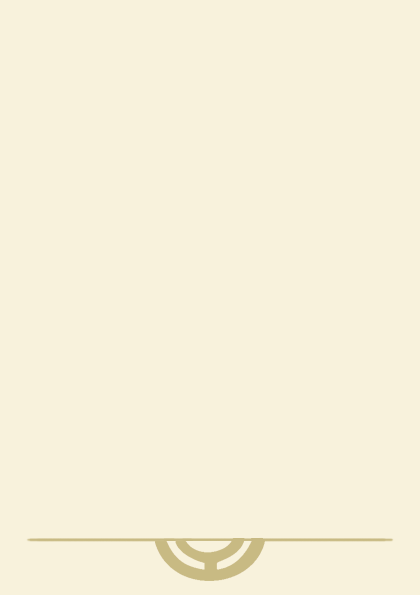
\includegraphics{下半示例.png}, center, scale=1, angle=0, opacity=1}
\BgThispage
\paragraph{实例 2} 对结构体进行排序。比如定义学生结构体,先按成绩从大到小排序,成绩相同的再按序号从小到大排序。
\begin{lstlisting}
#include<bits/stdc++.h>
using namespace std;
struct rec{  //定义学生结构体
    int id, score;
}student[101];
bool compare(rec x, rec y){ //定义排序规则
    if(x.score != y.score)
        return x.score > y.score; //先按成绩降序排序
    else
        return x.id < y.id; //成绩相同的再按序号升序排序
}

int main(){
	int n = 5;
	int scoreList[5] = {80,90,90,95,90};
	for(int i=1; i<=n; i++){ //对学生信息赋值
		student[i].id = i;
		student[i].score = scoreList[i-1];
	}
	sort(student+1, student+1+5, compare); //调用排序函数
	for(int i=1; i<=n; i++)
		printf("student %d: score: %d\n", student[i].id, student[i].score);
	return 0;
}
\end{lstlisting}


\end{document} 